\section{Architecture générale}
Le but du projet est de permettre à des applications de modifier des fichiers stockés à différents endroits, via le protocole défini par UbuntuOne.
Pour cela, plusieurs composants sont nécessaires :
\begin{itemize} 
   \item Le serveur : Le serveur reçoit des instructions via l'API d'UbuntuOne, par HTTP.
   \item Les clients : Les clients sont la partie utilisateur. Ces clients échangent avec le serveur via l'API. 
   \item Les drivers : Les drivers permettent d'échanger entre le serveur, et les différentes solutions de stockage. 
\end{itemize}

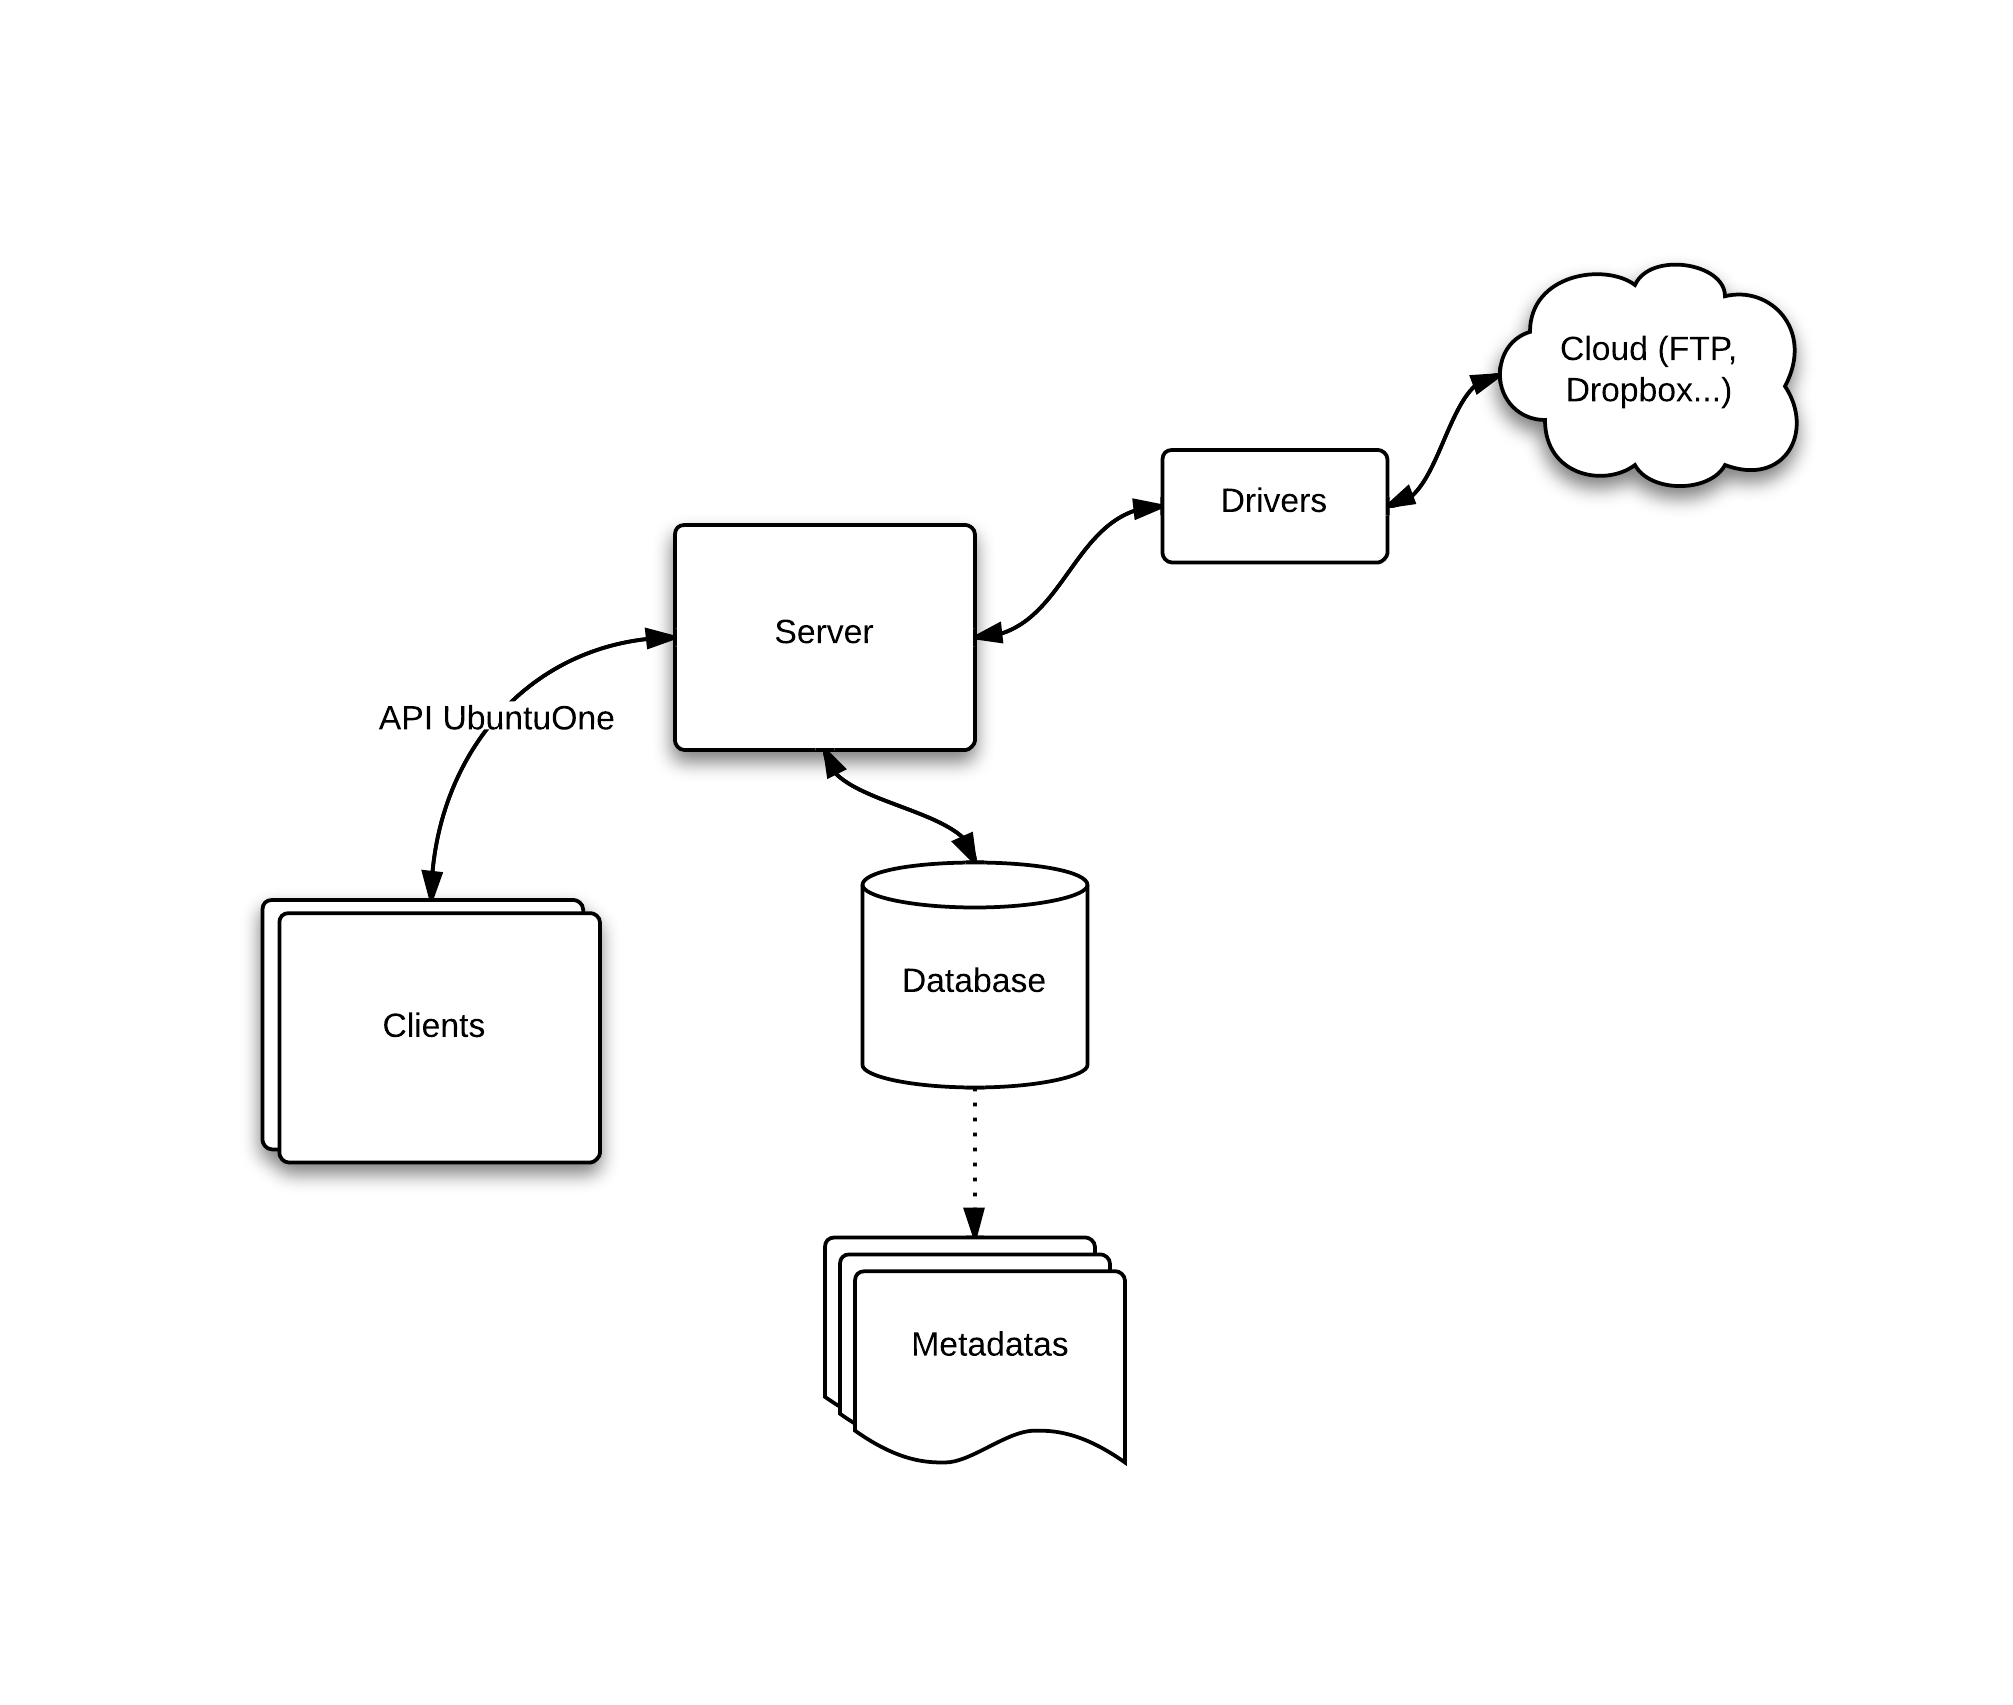
\includegraphics[width=500pt]{architecture.png}

\section{Serveur}
Le serveur est la partie centrale du projet. Il doit interpréter les instructions envoyés par les clients, et y répondre.

Une implémentation a été effectuée par l'entreprise Canonical, à l'origine d'UbuntuOne. Cette implémentation utilise les services de Cloud Computing EC2 et S3 d'Amazon. Suite à un partenariat entre ces deux entreprises, le code source du serveur n'est pas disponible, et ne le sera à priori jamais.

Notre serveur utilisera une base de données pour stocker les méta-données des fichiers.

Onitu permet aux utilisateurs de choisirs plusieurs moyens pour stocker leur données. Du point de vue du serveur, cela se fait grâce aux méta-données stockées en base de données, qui contiennent les informations nécessaires aux drivers pour récupérer les données. 

\section{Drivers}
Les drivers permettent la communication entre le serveur et les différentes solutions de stockage. Ils sont construits autour d'une interface commune, qu'ils étendent afin d'intéragir avec la solution à laquelle ils sont destinés.

Tous les drivers doivent permettre d'effectuer les quatre opérations de base : la création d'un fichier, sa récupération, son édition et sa suppression (connu sous l'accronyme CRUD, pour Create, Read, Update, Delete).

Du fait du côté ouvert d'Onitu, n'importe qui peut créer son propre driver. Ceci dit, plusieurs sont prévus et seront maintenus par l'équipe de développement :
\begin{itemize}
    \item Stockage local : Pour permettre de stocker des fichiers sur le serveur où est installé Onitu.
    \item Dropbox/Box.com/Google Drive/SkyDrive : Onitu pourra utiliser ces services tiers pour stocker les fichiers, si l'utilisateur possède un compte.
    \item (S)FTP/SSH/NFS/Webdav/Samba/HTTP : Des drivers seront dévelopés afin d'être compatible avec n'importe quel serveur supportant au moins un de ces protocoles.
    \item UbuntuOne : Il sera possible d'utiliser n'importe quel serveur compatible avec l'API d'UbuntuOne comme serveur de stockage.
\end{itemize}

\section{Clients}

\section{Interface Web}
